%%
%% 研究報告用スイッチ
%% [techreq]
%%
%% 欧文表記無しのスイッチ(etitle,jkeyword,eabstract,ekeywordは任意)
%% [noauthor]
%%

%\documentclass[submit,techreq]{ipsj}
\documentclass[submit,techreq]{ipsj}

\usepackage[dvips]{graphicx}
\usepackage{latexsym}
\usepackage{here} % [H]とするとその場所に配置されるらしい

\def\Underline{\setbox0\hbox\bgroup\let\\\endUnderline}
\def\endUnderline{\vphantom{y}\egroup\smash{\underline{\box0}}\\}
\def\|{\verb|}

%\setcounter{巻数}{53}%vol53=2012
%\setcounter{号数}{2}
%\setcounter{page}{1}

% インタラクション特有の設定。印刷工程で柱・ノンブルの埋め込みを行う。
\makeatletter
\pagestyle{empty}
\def\@oddhead{}%
\def\@evenhead{}%
\def\ps@IPSJTITLEheadings{}
\makeatother

\begin{document}

\title{降臨鉄道: 模型モノレールを利用した遠隔通信}
\etitle{Camera on Rails: Telecommunication with Model Monorail Trains}

\affiliate{KU}{慶應義塾大学 環境情報学部\\
Faculty of Environment and Infomation Studies, Keio University}

\author{山田 尚昭}{Naoaki Yamada}{KU}
\author{増井 俊之}{Toshiyuki Masui}{KU}

\begin{abstract}
% 現代では2ちゃんねる等に有名人が書き込みをすることが降臨と呼ばれており、降臨の
% 場では普段雲の上の存在である有名人が、その場の人々と親しく交流をしている.
% 我々はこのネット上の降臨を実世界に実現することで、研究室OBと現役学生のコミュ
% ニケーションを実現できるのではないかと考えた.さらに、天井を移動するモノレール
% 型の鉄道玩具を用いて、従来の遠隔コミュニケーションシステムには無い自由な移動と
% より広い視野を手に入れた.

カメラを登載した模型モノレールをオフィスの天井で走らせることによって、
オフィス外の人間がオフィス内の人間と会話することができるシステムを作成した。
車輪で移動可能なロボットを利用することによって
遠隔地のユーザがオフィスの会議などに参加する試みが近年盛んになっているが、
混雑した場所でロボットが自由に移動することは難しいことが多い。邪魔物が存在しない天井を自由に移動できる装置を利用することによって、
実用的な遠隔コミュニケーションシステムが実現できた。
本システムの利用により、
卒業したメンバが部室を訪れる「OB降臨」機能を手軽に実現することができる。
\end{abstract}

%\begin{jkeyword}
%情報処理学会論文誌ジャーナル,\LaTeX,スタイルファイル,べからず集
%\end{jkeyword}
%
\begin{eabstract}
We developed the ``Camera on Rails'' telecommunication system with
which people out of the office can communicate with people in the
office through a camera on a model monorail train running on the ceiling
of the office. Using the system, people can monitor the current status
of the office by running the train on the ceiling, and have
conversation with the people in the office.
\end{eabstract}
%
%\begin{ekeyword}
%IPSJ Journal, \LaTeX, style files, ``Dos and Dont's'' list
%\end{ekeyword}

\maketitle

%1
\section{はじめに}

遠隔地の人とあたかも同じ場所にいるかのような感覚を強化するテレプレゼンスの
システムの研究は盛んに行われている.今日ではビデオ会議システムや遠隔操作可能な
人間を模したロボットなどが普及しつつある.

以前に研究室では卓上を動き回ることのできるロボットを介した遠隔コミュニケーション
支援システムを製作したが\cite{Hirota:Korin},動ける範囲に制限があったり
障害物に阻まれてカメラからの映像が見られなかったりすることがあった.

何にも邪魔をされることのない部屋の天井を移動する遠隔情報共有システム
降臨鉄道を提案する.

%2
\section{関連研究}

Double RoboticsのDouble\footnote{
  \textsf{http://www.doublerobotics.com}
}
は遠隔地から操作可能な高さ約1.2mのテレプレゼンス
ロボットである.Doubleのような人間の分身を模したロボットは,卓上に置かれた
小型のロボットに比べて移動できる範囲は大きいが,他の人の邪魔になったりする
ことがある.

\begin{figure}[H]
\centerline{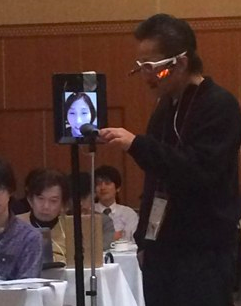
\includegraphics[width=60mm,bb=-100 0 241 306]{figures/b74f4564d4b38d12e48fcf80fef96def.png}}
\caption{WISS2014で質疑応答に利用されたDouble.}
\label{screenshot1}
\end{figure}

Jouppiのシステム\cite{Jouppi:2002:FST:587078.587128}では自由に動き回れるロボットで遠隔地を訪れられる.大掛かりな
操作室が必要だが、現地での活動能力は高い.

%3
\section{降臨鉄道}

ユーザはWebページにアクセスすることで降臨鉄道が設置された遠隔地のリアルタイム
映像を見たり,降臨鉄道を操作して移動させることができる(図\ref{monorail}).

\begin{figure}[H]
\begin{center}
\includegraphics[width=100mm,bb=-40 0 640 480]{figures/image.png}
\end{center}
\caption{天井を走る降臨鉄道.}
\label{monorail}
\end{figure}


降臨鉄道システムは,Androidスマートフォンが取り付けられた懸垂式モノレール型の
鉄道玩具「降臨鉄道」とWebサーバ,linda-serverから構成される.

降臨鉄道にはAndroidスマートフォンが搭載されており,サーバからの命令を受け取り
DCモータを制御する.DCモータの制御は440Hzの正弦波のMP3音声ファイルを再生し,
イヤホン端子から擬似的な交流電源を得てリレーを駆動させることによって行っている.
動画の配信にはAndroidアプリケーションIP Webcam\footnote{
  \textsf{https://play.google.com/store/apps/details?id=com.pas.webcam}
}
を使用し,MotionJPEG形式の
影像をHTTP通信で配信している.

WebサーバにはAndroid用のページとクライアント用のページが
用意されている(図\ref{browser}).

\begin{figure}[H]
\begin{center}
\includegraphics[width=120mm,bb=0 0 640 454]{figures/korin.png}
\end{center}
\caption{クライアントのWebサイト. モノレールからの映像が表示される.}
\label{browser}
\end{figure}

クライアント用ページでは降臨鉄道のカメラからの影像の表示と移動の命令をし,
Android用ページでは移動の命令に従って音声ファイルを再生している.

操作は並列計算プリミティブLinda\cite{Carriero:1989:LC:63334.63337}
Webサーバ上に実装したlinda-server\footnote{
  \textsf{https://github.com/node-linda/linda}
}
を用いて実装している.

%4
\section{まとめと展望}

% 遠隔イベント参加とか.
今回のデモで紹介したシステムは現在,研究室内で実際の運用を通じて実験中である.
降臨鉄道は多くの人が集まるイベント会場などで遠隔イベント参加システムとして利用
できると考える.

また,将来的には目的に応じたロボットを複数個用意し,世代間を超えてより活発な
研究活動ができるようにしたいと考えている.

% \begin{acknowledgment}
% 本研究に協力していただいた増井研のメンバーに感謝いたします.
% \end{acknowledgment}

\bibliographystyle{ipsjsort}
\bibliography{paper}

\end{document}
